%\emph{(En esta subsección se deben describir y justificar los metodos de desarrollo y/o investigación que se aplicaran a lo largo del desarrollo del proyecto.)}

%\emph{(La longitud máxima de esta sección es de 1 página.)}

La metodología a utilizar es la metodología de desarrollo ágil Melé\footnote{Desde la Séptima Edición del libro ``Ingenieria del software. Un enfoque practico.'' del Ph.D. Roger S. Pressman, es llamado Scrum }~\cite{7}.

Dicha metodología, tiene como objetivo guiar las actividades en un margen que incorpora las siguientes acciones del marco de trabajo: \emph{requisitos, análisis, diseño, evolución y entrega}. En cada actividad mencionada anteriormente, ocurren dentro de un proceso conocido como \emph{Sprint}. El beneficio que tiene el trabajo realizado dentro del proceso mencionado con anterioridad  es que se adapta al problema y con frecuencia se modifica en tiempo real.

\begin{figure}[!hb]
	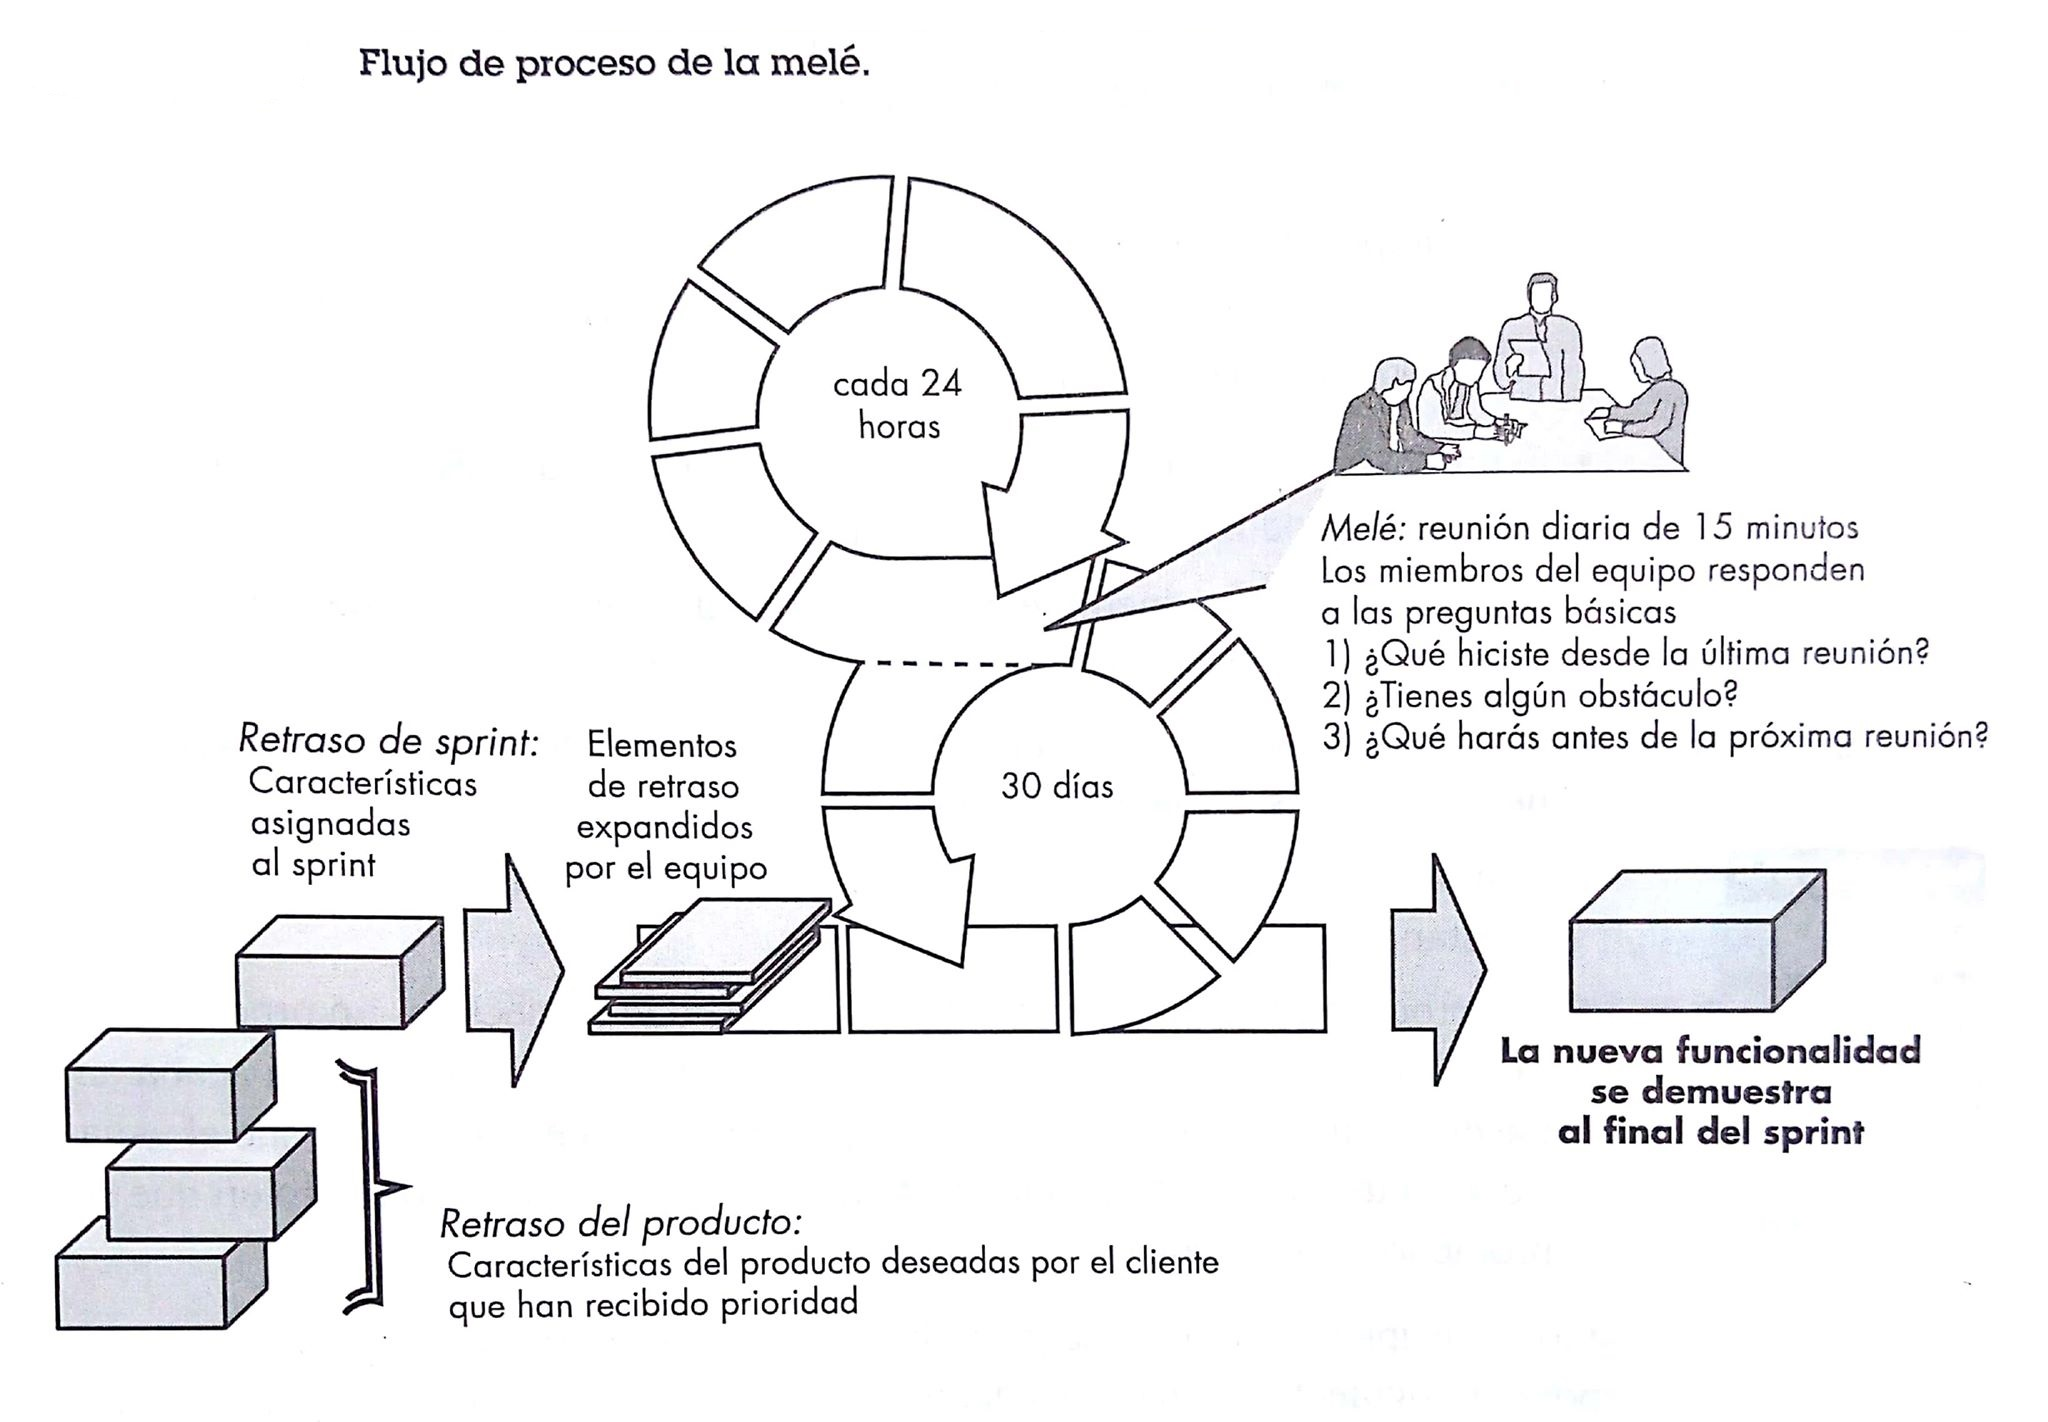
\includegraphics[width=\textwidth]{Imagenes/mele.jpg}
	\caption{\label{fig: procesoMele} Proceso de metodología Melé.}
\end{figure}

En la \textbf{Figura~\ref{fig: procesoMele}} se puede observar que Melé tiene un conjunto de \emph{``patrones de proceso de software''} los cuales define un conjunto de actividades de desarrollo:

\begin{itemize}
	\item 	\begin{description}
				\item[Retrasos:] lista de requisitos o características del proyecto ordenadas por prioridad, los cuales proporcionan valor comercial para el cliente. Además, en cualquier momento se pueden agregar elementos a los retrasos. Por otra parte, el gerente del proyecto, evalúa los retrasos y actualiza las prioridades de esta lista de acuerdo con lo requerido. 
			\end{description}

	\item 	\begin{description}
				\item[Sprint:] proceso por el cual se requiere satisfacer un requisito definido en los retrasos en un periodo predefinido (usualmente es de 30 días). Cuando se comienza un Sprint, no se pueden agregar nuevos cambios. Por lo tanto, esto permite trabajar en un ambiente enfocado a corto plazo, pero estable.
			\end{description}

	\item 	\begin{description}
			    \item[Reuniones:] juntas de corto periodo (por lo general 15 minutos) las cuales se realizan a diario por el equipo de Melé, en donde todos los miembros del equipo se deben plantear y responder las 3 siguientes preguntas: 

			    \begin{itemize}
			    	\item ¿Qué hiciste desde la última reunión?

			    	\item ¿Cuáles obstáculos encontraste? 

			    	\item ¿Qué esperas lograr para la siguiente reunión del equipo?
			    \end{itemize}

			 	Cada reunión ayuda a descubrir problemas potenciales tan pronto sea posible.
			\end{description}

	\item 	\begin{description}
				\item[Demostración:] entrega de incremento del software al cliente de tal manera que éste evalúe la funcionalidad implementada. Cabe destacar la posibilidad de que la demostración no contenga toda la funcionalidad planteada, sino que aquellas funciones susceptible de entregarse dentro del periodo establecido.
			\end{description}
\end{itemize}

Los motivos por los cuales se utiliza este método son:

\begin{itemize}
	\item Completa participación del cliente y prueba de funcionalidades para obtener retroalimentación.

	\item Se pueden obtener los cambios y adaptarse al proyecto en cada Sprint.

	\item Como la idea principal es realizar rendiciones y se han aclarado algunos requerimientos, mas no son todos, es que se espera que el proyecto aumente en el proceso de desarrollo. Es por esta incertidumbre que se escoge la metodología Melé, ya que ayuda al cliente y al equipo de trabajo a definir los requisitos del proyecto.
\end{itemize}

%\begin{figure}
%  \centering
%    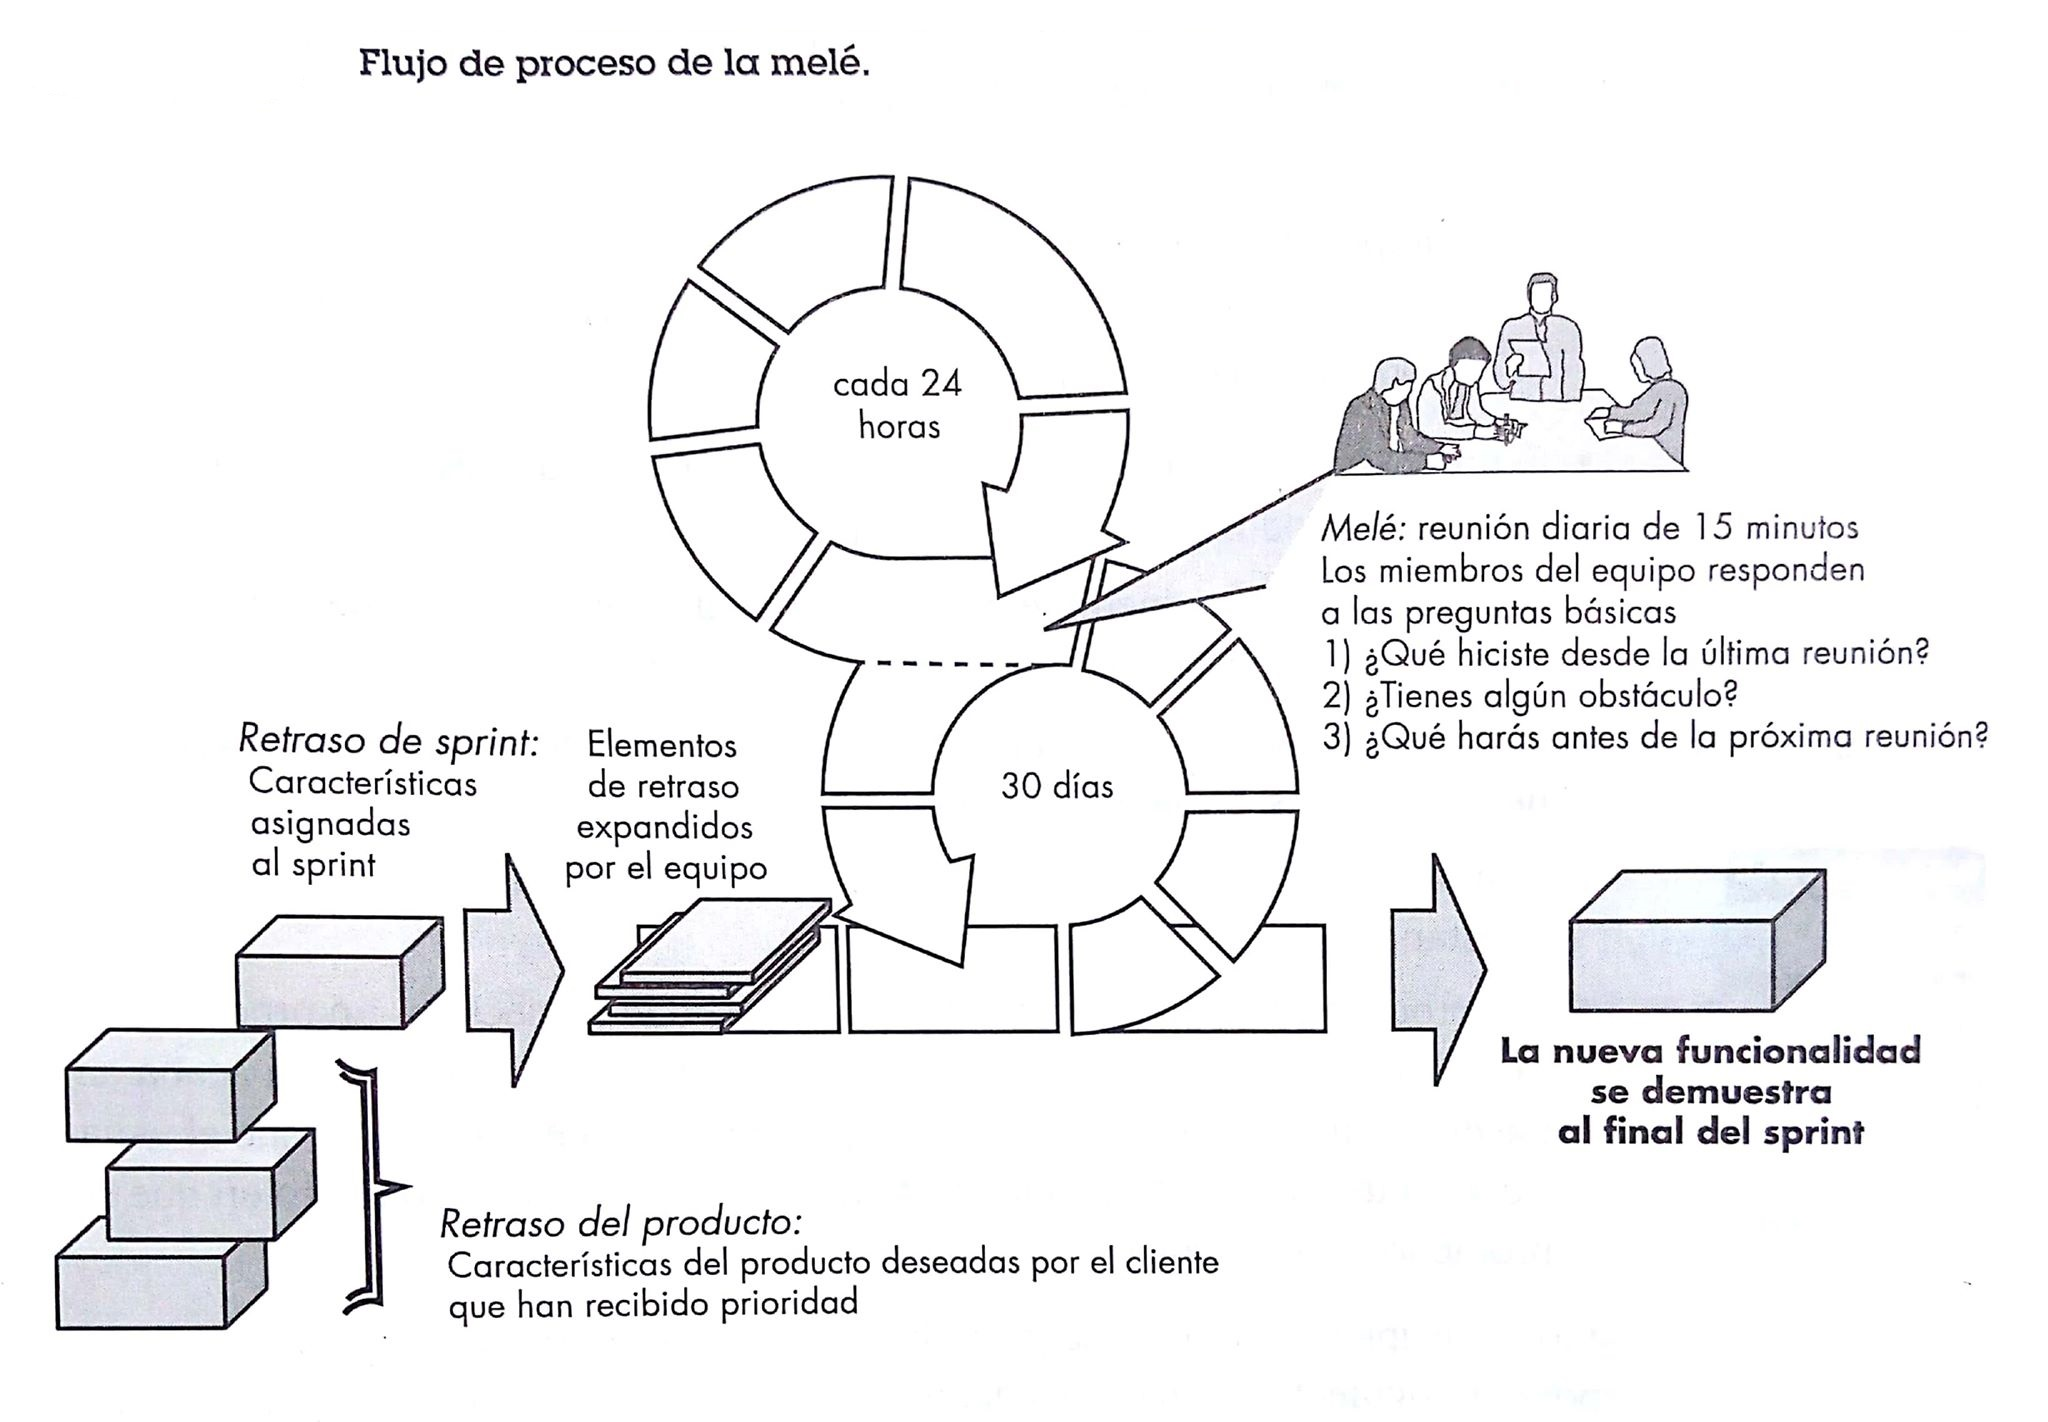
\includegraphics[width=1.2\textwidth]{Imagenes/mele.jpg}
%  \caption{Mi Figura}
%  \label{fig:ejemplo}
%\end{figure}
